\documentclass{article}

\usepackage{graphicx}
\usepackage{a4wide}

\title{The FieldTrip Multivariate Module}
\author{Marcel van Gerven}

\renewcommand{\t}[1]{{\tt #1}}

\begin{document}
\maketitle
\thispagestyle{empty}

\newpage

\tableofcontents

\newpage

\section{Module layout}

The FieldTrip Multivariate Module (FMM) is a generic machine learning toolbox with additional support for the analysis of neuroimaging datasets and is written in object-oriented Matlab. It is especially suitable for applications in Brain-Computer Interfacing (BCI) and multivariate pattern analysis (MVPA).

\begin{figure}[ht]
\begin{center}
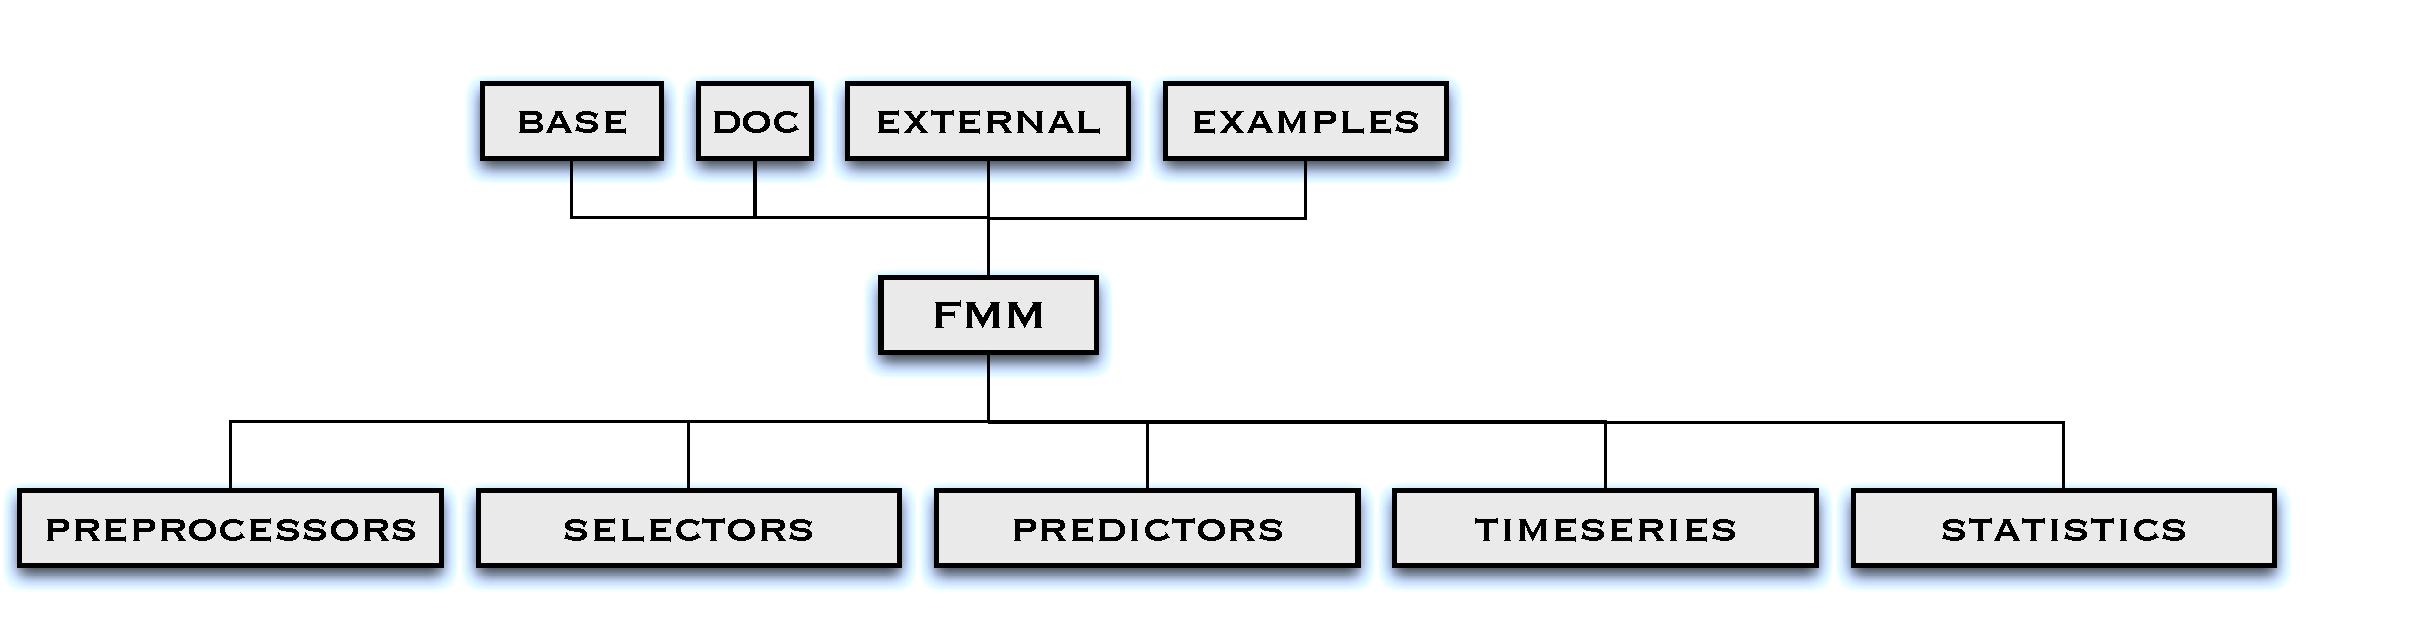
\includegraphics[width=\textwidth]{figures/organization.pdf}
\caption{FMM's directory structure}
\end{center}
\label{dir}
\end{figure}

The organization of FMM's directory structure is shown in Figure~\ref{dir}. The role of each directory is as follows:
\begin{itemize}
\item \t{base}: abstract classes that should not be used directly 
\item \t{preprocessors}: preprocessing wrapper classes
\item \t{selectors}: feature selection wrapper classes
\item \t{predictors}: prediction wrapper classes
\item \t{timeseries}: timeseries analysis wrapper classes
\item \t{statistics}: crossvalidation, performance measures, significance tests and parameter optimization
\item \t{doc}: FMM documentation
\item \t{external}: machine learning toolboxes used by wrapper classes
\item \t{examples}: example scripts and datasets
\end{itemize}

\begin{table}[ht]
\centering
\caption{External toolboxes.}
\begin{tabular}{l|l|l}
{\bf name} & {\bf function} & {\bf author}\\
\hline
bahramisharif & elastic net & Ali Bahramisharif  \\
farquhar & kernel methods & Jason Faquhar\\
gerven & Bayesian methods & Marcel van Gerven\\
glmnet & Fortran version of elastic net & Jerome Friedman\\
herman & common spatial pattern & Pawel Herman\\
L1General & L1 regularization & Mark Schmidt\\
murphy & LDS/HMM toolbox & Kevin Murphy\\
utilities & global functions & Marcel van Gerven
\end{tabular}
\label{tab:external}
\end{table}


The basic philosophy of FMM is that new methods can be added as toolboxes which are called through generic wrapper code. This makes it easy to extend the toolbox to fit your own needs. The currently used external toolboxes are listed in Table~\ref{tab:external}. Different multivariate methods can be concatenated together in a processing pipeline, constituting a multivariate analysis \t{ft\_mv\_analysis}, or MVA for short. Finally, an \t{ft\_mv\_analysis} object can either be used standalone or be evaluated on data using a \t{ft\_mv\_crossvalidator} object. This automates the whole process of analyzing (neuroimaging) data. Figure~\ref{class} shows a diagram of FMM classes, to which will be referred later on. 

\begin{figure}[ht]
\begin{center}
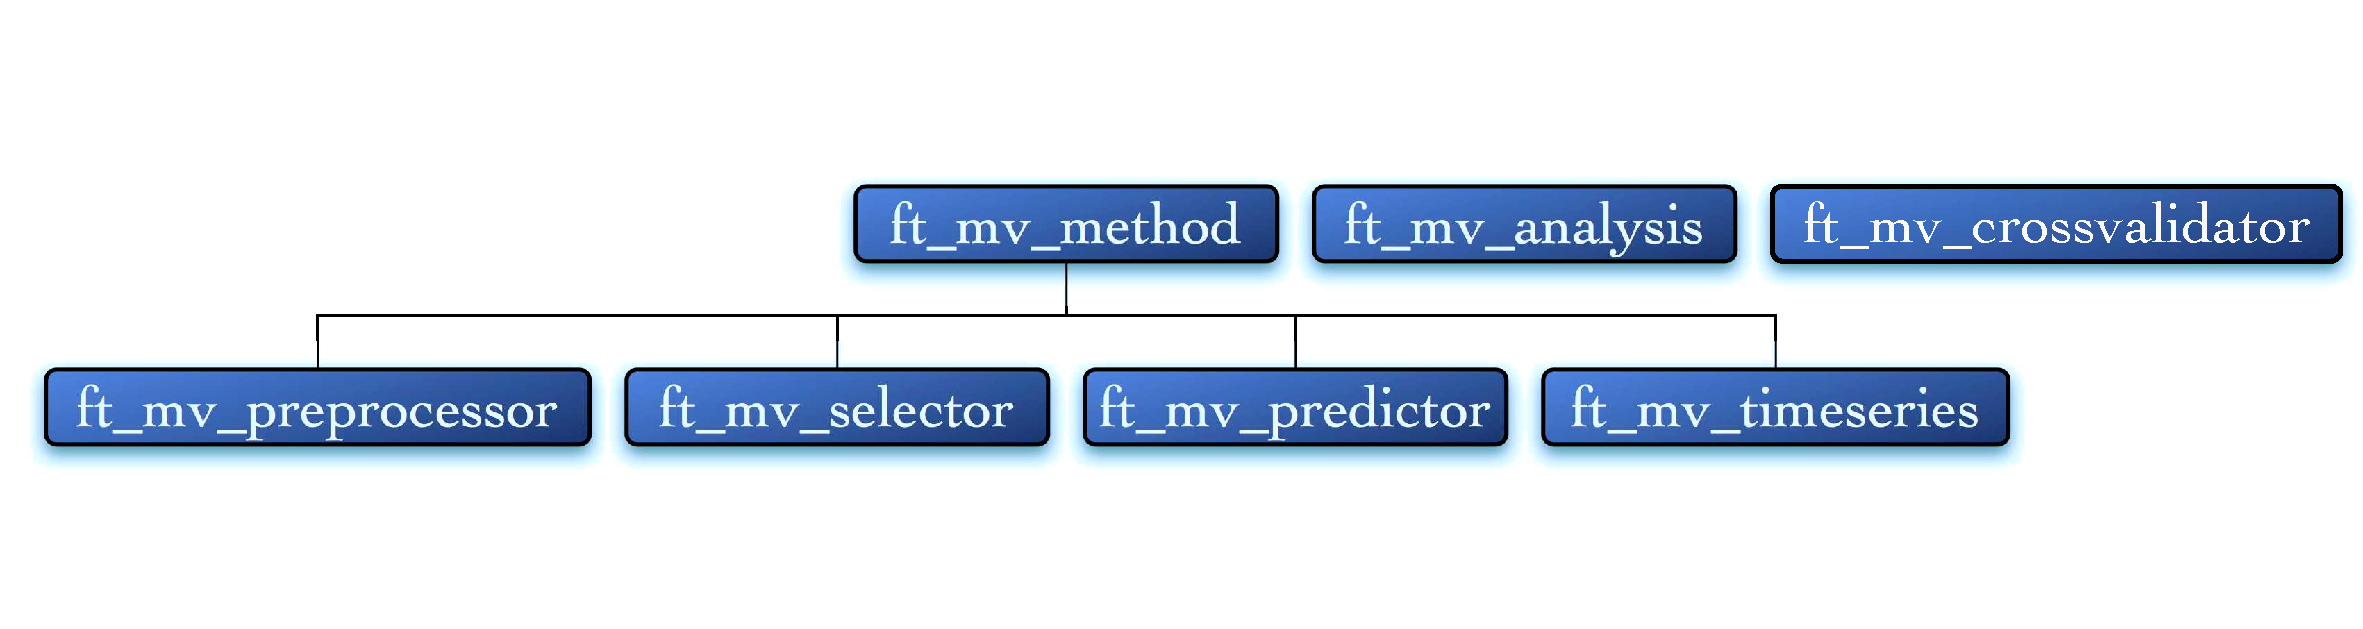
\includegraphics[width=\textwidth]{figures/classes.pdf}
\caption{FMM's class diagram}
\end{center}
\label{class}
\end{figure}

\newpage

\section{Data handling}

In FMM, a dataset is represented as a multidimensional array, where the first dimension indexes datapoints and the remaining dimensions are arbitrarily chosen. Multiple datasets are represented as a cell-array of multidimensional arrays. An exception to this rule holds for \t{ft\_mv\_timeseries} objects, where the first dimension indexes time and multiple timeseries are represented as a cell-array. Missing values are represented using \t{NaN}.

\section{Multivariate analysis}

A multivariate analysis is a Matlab object which can be constructed as follows:
\begin{verbatim}
obj = ft_mv_analysis({method1,...,methodN})
\end{verbatim}
where the argument is a cell-array of multivariate methods. By calling
\begin{verbatim}
obj.train(X,Y)
\end{verbatim}
we can train our MVA on input \t{X} and output \t{Y}. Finally, we can test on new data \t{U} by calling
\begin{verbatim}
V = obj.test(U)
\end{verbatim}
such that \t{V} contains the predictions. The MVA object will sequentially call each \t{ft\_mv\_method} in the pipeline where output of the previous method will be input to the next method. The \t{obj.name} will return the MVA as a string and the method \t{obj.model} will return the associated model, in this case the model of the last method in the pipeline (more on this later).

\newpage

\section{Multivariate methods}

Multivariate methods are organized into different subclasses according to the way they transform input data \t{X} to output data \t{Y}. Currently supported methods are {\em preprocessors}, which preprocess the data, {\em selectors}, which perform some kind of feature selection, {\em predictors}, which make predictions for new data, and {\em timeseries} methods, which perform timeseries analysis on the data. Many methods handle missing data, multiple outputs, multiple datasets and online (sample by sample) learning. If a method does not handle any of these situations then it will throw an error. Handling of some of these situations can be done by invoking a wrapper function.\footnote{E.g, multiple outputs can be handled by invoking an \t{ft\_mv\_noutput} object and multiple datasets can be handled by invoking the \t{ft\_mv\_ndata} object.}

All \t{mvmethod} classes are structured as follows (here we show an example of a predictor):
\begin{verbatim}
classdef mymethod < ft_mv_predictor
 
   properties % insert class-specific properties here
   end
 
   methods
 
        function obj = mymethod(varargin)       
         	obj = obj@ft_mv_predictor(varargin{:});
        end        
 
        function obj = train(obj,X,Y)
           % estimate mvmethod parameters
        end
 
        function Y = test(obj,X)
        	 % compute output     
        end
 	
        function X = invert(obj,Y)
        % optional function which inverts the mapping performed by this class
        
        end
 
        function [m,d] = model(obj)
          % return the model parameters as a cell-array m
          % desc contains a description of each element of m 
        end
    end
 
end
\end{verbatim}

In the following subsection we list the currently supported methods. More complete descriptions can be found in the help of the respective methods and examples of their use can be found in Section~\ref{examples}.

\subsection{Preprocessors}

Preprocessors are used to preprocess the input data \t{X} in such a way that it will be more suitable for making predictions. Table~\ref{preprocessors} lists the currently supported preprocessors and their functionality.

\begin{table}[ht]
\centering
\caption{Preprocessors}
\begin{tabular}{p{0.2\textwidth}|p{0.7\textwidth}}
\bf{preprocessor} & \bf{functionality}\\
\hline
\t{ft\_mv\_standardizer} &  centers and scales the data such that it has mean zero and a standard deviation of one\\
\t{ft\_mv\_whitener} & whitens the data\\
\t{ft\_mv\_csp} & common spatial pattern algorithm\\
\t{ft\_mv\_pca} & principal component analysis
\end{tabular}
\label{preprocessors}
\end{table}

\subsection{Selectors}

Selectors are used to perform feature selection on the input data \t{X}. Table~\ref{selectors} lists the currently supported selectors and their functionality.

\begin{table}[ht]
\centering
\caption{Selectors}
\begin{tabular}{p{0.2\textwidth}|p{0.7\textwidth}}
\bf{selector} & \bf{functionality}\\
\hline
\t{ft\_mv\_filterer} & Performs feature selection by computing a univariate measure for each feature and taking the best $N$ features based on a crossvalidator\\
\t{ft\_mv\_searchlight} & Performs a searchlight analysis
\end{tabular}
\label{selectors}
\end{table}

\subsection{Predictors}

Predictors are used to predict new outputs \t{Y} based on input data \t{X}. Table~\ref{predictors} lists the currently supported predictors and their functionality.

\begin{table}[ht]
\centering
\caption{Predictors}
\begin{tabular}{p{0.2\textwidth}|p{0.7\textwidth}}
\bf{predictor} & \bf{functionality}\\
\hline
\t{ft\_mv\_blogreg} & Bayesian logistic regression with a multivariate Laplace prior\\
\t{ft\_mv\_naive} & Naive Bayes classifier with normally distributed feature values\\
\t{ft\_mv\_svm} & Support vector machine; inherits from \t{ft\_mv\_kernelmethod}\\
\t{ft\_mv\_klr}  &  Kernel logistic regression;  inherits from \t{ft\_mv\_kernelmethod}\\
\t{ft\_mv\_rfda} & Regularized Fisher discriminant analysis\\
\t{ft\_mv\_logreg} & Logistic regression with L1 and/or L2 regularization\\
\t{ft\_mv\_glmnet} & Wrapper class for efficient implementation of elastic net linear and logistic regression\\
\t{ft\_mv\_linreg} & Linear regression with L1 and/or L2 regularization\\
\t{ft\_mv\_rkls} & Regularized kernel least squares; inherits from \t{ft\_mv\_kernelmethod}\\
\t{ft\_mv\_rls} & Recursive least squares regression\\
\t{ft\_mv\_ensemble} & Ensemble method class that uses multiple mvmethods in parallel to achieve some goal
\end{tabular}
\label{predictors}
\end{table}

\subsection{Timeseries}

Timeseries methods are used to predict new outputs \t{Y} based on input data \t{X} whose first dimension indexes time. Table~\ref{timeseries} lists the currently supported timeseries analysis methods and their functionality.

\begin{table}[ht]
\centering
\caption{Timeseries analysis methods}
\begin{tabular}{p{0.2\textwidth}|p{0.7\textwidth}}
\bf{timeseries} & \bf{functionality}\\
\hline
\t{ft\_mv\_hmm} & Hidden Markov model\\
\t{ft\_mv\_lds} & Linear dynamical system
\end{tabular}
\label{timeseries}
\end{table}

\subsection{Classification, regression and MIMO models}

Note that the above predictors can perform classification tasks, regression tasks or represent multiple-input multiple-output (MIMO) models. In case of K-class classification, it is assumed that the output vector Y consists of labels $1:K$. For example, $Y = [2\,1\, 1\, 2\, 1\, 2]'$ assigns examples 2, 3 and 5 to class 1 and the remaining examples to class 2. In case of regression, $Y$ just consists of the observed real output per example. In case of MIMO models , the same behaviour holds, but $Y$ consists of multiple columns where each column stands for a separate variable.

\subsection{Grid search}

For many of the described methods there are free parameters which need to be optimized. For instance, the $C$ parameter of the SVM or  the regularization parameters $L1$ and $L2$ for the elastic net.  In those cases, it is useful to employ the \t{ft\_mv\_gridsearch}.  This object can be used to optimize free parameters of a multivariate analysis in a fully automated way. The grid search is called as folllows:
\begin{verbatim}
ft_mv_gridsearch('mva',mymva,'validator',ft_mv_crossvalidator...
	('metric',mymetric),'mvidx',myidx,'vars',myvars,'vals',myvals)
\end{verbatim}
where \t{mymva} is the employed MVA, \t{mymetric} the employed performance measure to test which configuration is optimal, \t{myidx} the index of the method in \t{mymva} that is to be optimized, \t{myvars} the variable of mymva{myidx} that needs to be optimized and \t{myvals} the values which that variable may assume. This sounds complicated but it is not. Let's clarify with some examples. Suppose we wish to optimize the $C$ parameter of an SVM in the range \t{logspace(-3,3,7)}. Then, we can use 
\begin{verbatim}
% crossvalidator with 80% of the data and accuracy as the metric
cv = ft_mv_crossvalidator('nfolds',0.8,'metric','accuracy'); 

opt = ft_mv_gridsearch('verbose',true,'mva',svm,'validator',cv,...
'vars','C','vals',logspace(-3,3,7))

% standard behavior from here on
opt = opt.train(X,Y) 
...
\end{verbatim}


% crossvalidate
% evaluate
% significance

% optimizer 
% ensemble
% one-against-one etc



\subsection{Ensemble methods}

Ensemble methods evoke methods in parallel and combine their outputs in some prespecified way. In FMM this is realized through the \t{ensemble} object. For example, we can apply a naive Bayes classifier and a support vector machine through ensemble methods as follows:
\begin{verbatim}
m = ft_mv_ensemble('mvas',{ft_mv_naive ft_mv_svm},'combfun',myfun);
m = m.train(X,Y);
...
\end{verbatim}
Here, the user-specified function \t{myfun} specifies how the ouputs of naive Bayes and the SVM should be combined. For example, \t{myfun} could implement a majority vote as follows
\begin{verbatim}
function y = myfun(x)

  y = zeros(size(x{1}));
  for k=1:length(x)
      [temp,pcls] = max(x{k},[],2);
      for p=1:length(pcls)
         y(p,pcls(p)) = y(p,pcls(p)) + 1;
       end
   end
            
   % resolve ties
   for p=1:size(y,1)
    m = find(ismember(y(p,:),max(y(p,:))));
    y(p,:) = 0;
    if length(m) > 1
     m = m(ceil(rand*length(m)));
    end
    y(p,m) = 1;
  end
\end{verbatim}


\subsection{Multitask learning}

Multitask learning is the the notion that if we have multiple datasets (e.g., subjects, sessions) then we can learn better models for each dataset by being informed by the other datasets. For instance, if multiple datasets are given to \t{ft\_mv\_blogreg} then the same features are coupled between the different datasets. This leads to dataset-specific models that are easier to compare~\cite{gerven2010b}. For instance, in the following example we apply this method to two datasets, both generated by adding random noise to the original data.
\begin{verbatim}
>> load 69digits;
>> X1 = X + 0.05*randn(size(X));
>> X2 = X + 0.1*randn(size(X));
>> a = ft_mv_test('mva',{ft_mv_blogreg},'X',X1,'Y',Y);
>> disp(a)
    0.6600
>> a = ft_mv_test('mva',{ft_mv_blogreg},'X',X2,'Y',Y);
>> disp(a)
    0.5800
>> a = ft_mv_test('mva',{ft_mv_blogreg('taskcoupling',100)},'X',{X1 X2},'Y',Y);
>> disp(a)
    [0.6900]
    [0.5900]
\end{verbatim}
Hence, if we apply multitask learning then the results per dataset are influenced by the other datasets. The taskcoupling parameter effectively couples the models:
\begin{verbatim}
>> disp(corr(d.model{1,1},d.model{1,2}))
   0.9999
\end{verbatim}
Weaker coupling will cause weaker correlations between the models.

\newpage

\section{Statistics}

We can either use a MVA to perform online state estimation or to perform an offline analysis of neuroimaging data. The former is used in BCI applications (prediction) whereas the latter is used in offline analysis of BCI data or MVPA (model inference). Online state estimation is handled in the next section. Here, we describe statistics for models learned on offline data.

\subsection{Cross-validation}

Suppose we have acquired an offline dataset where subjects had to attend to the left or right visual field. In a MVPA approach, we want to get an estimate of how well our MVA can predict the attended location in individual trials and which features (brain regions, channels, latencies, frequencies, etc) contributed to this prediction. This can be assessed using the \t{ft\_mv\_crossvalidator} object. It splits the data into separate folds and learns for each fold a model on the remaining folds. For example, in case of ten-fold cross-validation we will obtain ten different models which are evaluated on ten different parts of the data. It is quite easy to perform such an analysis using FFM, as shown below.
\begin{verbatim}
% create crossvalidator object which 
% standardizes the data and applies an svm
cv = ft_mv_crossvalidator('mva',{ft_mv_standardizer ft_mv_svm});

% train cv on input data X and output data Y
cv = cv.train(X,Y);

% display classification accuracy
cv.metric = 'accuracy';
disp(cv.performance);
>> 0.80 % 80% correctly classified

% display outcome of mcnemar test
cv.sigtest = 'mcnemar';
disp(cv.significance);
>> 1e-4 % p-value; null-hypothesis rejected
\end{verbatim}
In the example, a ten-fold cross-validation is performed by standardizing the data and applying a support vector machine. Subsequently, the classification accuracy (proportion of correctly classified trials) is computed. Finally, an approximate binomial test (McNemar test) is computed which compares the predictions with that of a naive classifier that assigns all outcomes to the majority class. The different performance measures and significance tests can be examined by consulting the help for \t{ft\_mv\_performance} and \t{ft\_mv\_significance}. 

One may change \t{nfolds} to any number of folds, with \t{nfolds = inf} implementing leave-one-out cross-validation. Specifying a proportion for \t{nfolds} will use that proportion for training and the remaining data for testing. Finally, specifying \t{nfolds = 'online'} will simulate an online session by taking all trials in sequence where we train on trials $1,\ldots,n$ and test on trial $n+1$ for $n=0,\ldots,N-1$.

We have not yet mentioned how to determine which features were responsible for the predictions. This is realized throught the \t{model} field of the cross-validator. It returns the average model that is produced by the last method in the specified MVA; in our case, the model of a SVM. It is up to each multivariate method to  specify how its model is defined. For example, for the above example, assuming we used only five features, we have:
\begin{verbatim}

disp(cv.model);
>> [ 0.0176 -0.0305 0.0445 0.0904 0.0710]

disp(cv.description)
>> 'primal form parameters; positive values indicate condition 2'

\end{verbatim}

Supported performance measures and statistical tests are described in Tables~\ref{tab:measure} and \ref{tab:test}.
\begin{table}[ht]
\centering
\caption{Performance measures.}
\begin{tabular}{p{0.2\textwidth}|p{0.7\textwidth}}
{\bf measure} & {\bf output}\\
\hline
accuracy &proportion of correctly classified cases\\
contingency & contingency table with true class as rows and predicted class as colums\\
cfmatrix & confusion matrix with true class as rows and predicted class as colums\\
correlation & correlation between real and predicted output\\
invresvar & inverse residual variance
\end{tabular}
\label{tab:measure}
\end{table}

\begin{table}[ht]
\centering
\caption{Statistical tests.}
\begin{tabular}{p{0.2\textwidth}|p{0.7\textwidth}}
{\bf test} & {\bf output}\\
\hline
mcnemar & approximate binomial test
\end{tabular}
\label{tab:test}
\end{table}

\newpage

\section{Online state estimation}

If we use the toolbox for prediction then we need to work under strict time constraints. During training we want an optimal MVA to be learned quickly and be able to update our MVA with new incoming data. During testing we want to obtain an MVA output fast such that the online system does not stall. In the following example, we show an example of how online training and testing is realized.
\begin{verbatim}
% create a naive Bayes classifier
clf = ft_mv_naive

% train on initial data
clf = clf.train(X1,Y1)

% get output for new data; produces a posterior over classes
out1 = clf.test(x1);

% train some more (update the trained classifier)
clf = clf.train(X2,Y2);

% get output for new data; produces a posterior over classes
out2 = clf.test(x2);
\end{verbatim}
In the above example we used a naive Bayes classifier but the MVA can be arbitrarily complex. For example, 
\begin{verbatim}
clf = ft_mv_analysis({ft_mv_standardizer ...
        ft_mv_filterer('maxfeatures',10) ft_mv_svm})
\end{verbatim}
creates a MVA which first standardizes the data, then performs feature selection and finally applies a support vector machine.

\newpage

\section{Parallelization}
\label{parallel}

Some of the described methods can be resource intensive. Most notably, cross-validation, optimization, feature selection and the application of ensemble methods since they all require iterating over a collection of multivariate analyses. These methods all support parallel computing as implemented through FieldTrip's peer distributed computing module.

\newpage

\section{Examples}
\label{examples}

In the following examples, we will use the \t{69digits} dataset which is included in this module. It is a subset of the data used in~\cite{gerven2010,gerven2010a}. It consists of the BOLD measurements for 50 handwritten sixes and 50 handwritten nines as shown in a 3T MRI scanner. The dataset consists of the BOLD data \t{X}, the labels \t{Y} (1 stands for 6 and 2 stands for 9) and \t{images} (the presented handwritten digits). The variables \t{funloc} an \t{masks} contain the functional localizers and the associated mask in native space. The data pertains to the primary mask but subsets of features may be selected by using the other masks. In order to test a multivariate analysis we can make use of \t{ft\_mv\_test}. It accepts an MVA and tests it by default on the example dataset using ten-fold cross-validation.

\subsubsection*{A simple example}
We start with a simple example to get some baseline performance:
\begin{verbatim}
>> [a,b,c] = ft_mv_test('mva',{ft_mv_standardizer ft_mv_svm});
using default dataset 69digits
initializing random number generator with seed 1
validating 1 dataset(s)
input 1 consists of 100 examples and 569 features
output 1 consists of 100 examples and 1 features
validating using 10-fold cross-validation
using 10 folds for 1 datasets
dataset 1: validating fold 1 of 10 using 90 training samples and 10 test samples
dataset 1: validating fold 2 of 10 using 90 training samples and 10 test samples
dataset 1: validating fold 3 of 10 using 90 training samples and 10 test samples
dataset 1: validating fold 4 of 10 using 90 training samples and 10 test samples
dataset 1: validating fold 5 of 10 using 90 training samples and 10 test samples
dataset 1: validating fold 6 of 10 using 90 training samples and 10 test samples
dataset 1: validating fold 7 of 10 using 90 training samples and 10 test samples
dataset 1: validating fold 8 of 10 using 90 training samples and 10 test samples
dataset 1: validating fold 9 of 10 using 90 training samples and 10 test samples
dataset 1: validating fold 10 of 10 using 90 training samples and 10 test samples

>> disp(a)
    0.8300

>> disp(b)
     1.1050e-05

\end{verbatim}
Hence, baseline performance with a non-optimized SVM is 78\% of the trials classified correctly (output a) which is signficant as the null-hypothesis is rejected (output b). Output c returns the employed cross-validator.

\subsubsection*{Using the grid search}

In case we want to optimize the SVM then we can use \t{ft\_mv\_gridsearch}:
\begin{verbatim}
>> [a,b] = ft_mv_test('mva',{ft_mv_standardizer 
      ft_mv_gridsearch('mva',{ft_mv_svm},'vars','C','vals',logspace(-3,3,7))});

\end{verbatim}
Here we may obtain performance increases by searching over values for the $C$ parameter. Computing time in this case is about  300 times longer. The reason for this is that for each value in the search (seven in this case) it performs an inner ten-fold cross-validation within each outer cross-validation run. That is, we need to perform $7 \cdot 10 \cdot 10=700$ instead of $10$ SVM estimations. There are various ways to speed this up. For one, we can use less outer and inner folds for cross-validation (or even just a percentage of the data). Furthermore, we can parallelize the outer and inner cross-validation as well as the optimization. Note however that if we parallelize everything then the cluster may be too busy with broadcasting events instead of doing the actual computations! The optimal combination often is more an art than a science.

\subsubsection*{Using a predictor to combine ensemble method output}
It can be of interest to use the output of several predictors as input to another predictor. This is realized as follows:
\begin{verbatim}
m = ft_mv_ensemble('mvas',{ft_mv_naive ft_mv_svm},'combfun',@(x)(cell2mat(x)));
a = ft_mv_test('mva',{ft_mv_standardizer m ft_mv_naive});
\end{verbatim}

\subsubsection*{Using the searchlight method}

In this example, we show how we can compute the performance of individual spheres in a searchlight method using the default dataset. Note that we use a separate predictor within each sphere instead of the Mahalanobis distance as used by Kriegeskorte et al.
\begin{verbatim}
load 69digits;
\end{verbatim}
We first need to specify a cross-validator with which to test performance. We compute accuracy and a McNemar significance test by training on 80\% of the data and testing on 20\% of the data:
\begin{verbatim}
cv = ft_mv_crossvalidator('nfolds',0.8,'mva',{ft_mv_standardizer ft_mv_naive},...
           'metric','accuracy','sigtest','mcnemar');
\end{verbatim}
Now we may specify the searchlight. We need to specify the sphere radius and the step size. Furthermore, we may use a logical mask which specifies how where the used data features are in native space (e.g., when using a region of interest as in case of the default dataset). Finally, we need to specify the original dimensions of the input data (in this case the size of the mask). The searchlight will use the cross-validator to test performance in each sphere:
\begin{verbatim}
sl = ft_mv_searchlight('radius',3,'step',3,'mask',zmask,'validator',cv,'...
        indims',size(zmask),'verbose',true);
sl = sl.train(X,Y);
>> sl = sl.train(X,Y);
estimating 39 spheres with radius 3 with 3 steps for a...
volume of size [110  110   37]
estimating sphere 1 of 39
estimating sphere 2 of 39
estimating sphere 3 of 39
estimating sphere 4 of 39
...
average sphere volume: 52.2308
performance for sphere 1 of 39: 0.736842 (p-value: 0.342782)
performance for sphere 2 of 39: 0.842105 (p-value: 0.148915)
performance for sphere 3 of 39: 0.789474 (p-value: 0.267257)
performance for sphere 4 of 39: 0.684211 (p-value: 0.546494)
performance for sphere 5 of 39: 0.421053 (p-value: 0.75183)
performance for sphere 6 of 39: 0.736842 (p-value: 0.386476)
performance for sphere 7 of 39: 0.578947 (p-value: 1)
performance for sphere 8 of 39: 0.736842 (p-value: 0.342782)
performance for sphere 9 of 39: 0.578947 (p-value: 1)
performance for sphere 10 of 39: 0.684211 (p-value: 0.504985)
...
\end{verbatim}
In order to check how well each data feature  does in discriminating the classes, we may call \t{sl.model}. This projects back the average sphere results in native space.


\newpage

\section{References}

\bibliographystyle{plain}
\def\refname{}
\bibliography{/Users/marcelge/Documents/bibtex/mybibliography.bib,/Users/marcelge/Documents/bibtex/self.bib}

\end{document}